\documentclass[10pt,handout]{beamer}\usepackage[]{graphicx}\usepackage[]{color}
% maxwidth is the original width if it is less than linewidth
% otherwise use linewidth (to make sure the graphics do not exceed the margin)
\makeatletter
\def\maxwidth{ %
  \ifdim\Gin@nat@width>\linewidth
    \linewidth
  \else
    \Gin@nat@width
  \fi
}
\makeatother

\definecolor{fgcolor}{rgb}{0.345, 0.345, 0.345}
\newcommand{\hlnum}[1]{\textcolor[rgb]{0.686,0.059,0.569}{#1}}%
\newcommand{\hlstr}[1]{\textcolor[rgb]{0.192,0.494,0.8}{#1}}%
\newcommand{\hlcom}[1]{\textcolor[rgb]{0.678,0.584,0.686}{\textit{#1}}}%
\newcommand{\hlopt}[1]{\textcolor[rgb]{0,0,0}{#1}}%
\newcommand{\hlstd}[1]{\textcolor[rgb]{0.345,0.345,0.345}{#1}}%
\newcommand{\hlkwa}[1]{\textcolor[rgb]{0.161,0.373,0.58}{\textbf{#1}}}%
\newcommand{\hlkwb}[1]{\textcolor[rgb]{0.69,0.353,0.396}{#1}}%
\newcommand{\hlkwc}[1]{\textcolor[rgb]{0.333,0.667,0.333}{#1}}%
\newcommand{\hlkwd}[1]{\textcolor[rgb]{0.737,0.353,0.396}{\textbf{#1}}}%
\let\hlipl\hlkwb

\usepackage{framed}
\makeatletter
\newenvironment{kframe}{%
 \def\at@end@of@kframe{}%
 \ifinner\ifhmode%
  \def\at@end@of@kframe{\end{minipage}}%
  \begin{minipage}{\columnwidth}%
 \fi\fi%
 \def\FrameCommand##1{\hskip\@totalleftmargin \hskip-\fboxsep
 \colorbox{shadecolor}{##1}\hskip-\fboxsep
     % There is no \\@totalrightmargin, so:
     \hskip-\linewidth \hskip-\@totalleftmargin \hskip\columnwidth}%
 \MakeFramed {\advance\hsize-\width
   \@totalleftmargin\z@ \linewidth\hsize
   \@setminipage}}%
 {\par\unskip\endMakeFramed%
 \at@end@of@kframe}
\makeatother

\definecolor{shadecolor}{rgb}{.97, .97, .97}
\definecolor{messagecolor}{rgb}{0, 0, 0}
\definecolor{warningcolor}{rgb}{1, 0, 1}
\definecolor{errorcolor}{rgb}{1, 0, 0}
\newenvironment{knitrout}{}{} % an empty environment to be redefined in TeX

\usepackage{alltt}


%\usepackage{default}
\usepackage{animate} %need the animate.sty file 
\usepackage{graphicx}
%\graphicspath{{/home/sahir/Dropbox/jobs/laval/minicours/slides/}}
\usepackage{hyperref, url}
%\usepackage[round,sort]{natbib}   % bibliography omit 'round' option if you prefer square brackets
%\bibliographystyle{apalike}
\usepackage{biblatex}
\bibliography{bib.bib}
% Removes icon in bibliography
\setbeamertemplate{bibliography item}[text]

\usepackage[normalem]{ulem}

\setbeamertemplate{theorems}[numbered]

\setbeamertemplate{caption}[numbered]
\setbeamertemplate{caption label separator}{: }
\setbeamercolor{caption name}{fg=normal text.fg}

%\newtheorem{prop}{Proposition}
%\newenvironment{theoremc}[1]
%{\begin{shaded}\begin{theorem}[#1]}
%		{\end{theorem}\end{shaded}}
	
%\newtheorem{examplefirst}{Example}
%\newtheorem{examplesecond}{Example}
%\newenvironment<>{examplefirst}[1][]{%
%	\setbeamercolor{block title example}{bg=lightgray}%
%	\begin{example}#2[#1]}{\end{example}}
%\newenvironment<>{examplesecond}[1][]{%
%	\setbeamercolor{block title example}{fg=white,bg=blue!75!black}%
%	\begin{example}#2[#1]}{\end{example}}	

%\usepackage{amsthm}


\usepackage[figurename=Fig.]{caption}
\usepackage{subfig}
\usepackage{tikz, pgfplots,epsfig}
\usetikzlibrary{arrows,shapes.geometric}
\usepackage{color, colortbl,xcolor}
\definecolor{lightgray}{RGB}{200,200,200}
\definecolor{palegray}{RGB}{221,221,221}
\definecolor{myblue}{RGB}{0,89,179}
\definecolor{myorange}{rgb}{0.776,0.357,0.157}

\definecolor{gray}{RGB}{110,110,110}
\definecolor{darkgray}{RGB}{100,100,100}
\definecolor{lightgray}{RGB}{200,200,200}
\definecolor{turquoise}{RGB}{81,193,188}
\definecolor{tomato}{RGB}{255,136,136}
\definecolor{mandarina}{RGB}{229,169,25}
\definecolor{foreground}{RGB}{81,141,193}
\definecolor{background}{RGB}{246,244,240}
\definecolor{highlight}{RGB}{229,169,25}
\definecolor{lowlight}{RGB}{200,200,200}
\definecolor{beige}{RGB}{255,255,240}
\definecolor{pinkish}{RGB}{255,223,247}

\newcommand{\code}[1]{\texttt{#1}}


\usepackage{comment}
\setbeamercolor{frametitle}{fg=myblue}
\setbeamercolor{section in head/foot}{bg=myblue, fg=white}
\setbeamercolor{author in head/foot}{bg=myblue}
\setbeamercolor{date in head/foot}{bg=myblue}

\usepackage{amsthm}
\usepackage{shadethm}
%\colorlet{shadecolor}{blue!15}
\colorlet{shadecolor}{palegray}
%\setlength{\shadeboxrule}{.4pt}

%\newshadetheorem{thm}{Theorem}
\newshadetheorem{defm}{Definition}
\newshadetheorem{exm}{Exercise}
\newshadetheorem{remarkm}{Remark}
%\definecolor{shadethmcolor}{HTML}{EDF8FF}
\definecolor{shadethmcolor}{RGB}{221,221,221}
%\definecolor{shaderulecolor}{HTML}{45CFFF}
\definecolor{shaderulecolor}{RGB}{0,89,179}
\setlength{\shadeboxrule}{.4pt}

\newtheorem{thm}{Theorem}
\newcommand{\statetheoremhoriz}[2][\textwidth]{
	\par\noindent\tikzstyle{mybox} = [draw=myblue,left color=cyan!50,
	right color=cyan!5,thick,rectangle,inner sep=6pt]
	\begin{tikzpicture}
	\node [mybox] (box){%
		\begin{minipage}{#1}{#2}\end{minipage}
	};
	\end{tikzpicture}
}
\newcommand{\statetheoremvert}[2][\textwidth]{
	\par\noindent\tikzstyle{mybox} = [draw=myblue,top color=cyan!50,
	bottom color=cyan!5,thick,rectangle,inner sep=6pt]
	\begin{tikzpicture}
	\node [mybox] (box){%
		\begin{minipage}{#1}{#2}\end{minipage}
	};
	\end{tikzpicture}
}
\newcommand{\statetheoremsolid}[2][\textwidth]{
	\par\noindent\tikzstyle{mybox} = [draw=myblue,fill=palegray,
	thick,rectangle,inner sep=6pt]
	\begin{tikzpicture}
	\node [mybox] (box){%
		\begin{minipage}{#1}{#2}\end{minipage}
	};
	\end{tikzpicture}
}

\usetikzlibrary{shapes.geometric, arrows,shapes.symbols,decorations.pathreplacing}
\tikzstyle{startstop} = [rectangle, rounded corners, minimum width=3cm, minimum height=1cm, draw=black, fill=pinkish,text width=3.5cm]
\tikzstyle{startstop2} = [rectangle, rounded corners, minimum width=3cm, minimum height=1cm, draw=black, fill=background,text width=4.5cm]
\tikzstyle{startstop3} = [rectangle, rounded corners, minimum width=3cm, minimum height=1cm, draw=black, fill=beige,text width=3.0cm]
\tikzstyle{startstop4} = [rectangle, rounded corners, minimum width=3cm, minimum height=1cm, draw=black, fill=pinkish,text width=4.5cm]
\tikzstyle{io} = [trapezium, trapezium left angle=70, trapezium right angle=110, minimum width=2cm, minimum height=1cm, text centered, draw=black, fill=blue!30,text width=1.5cm]
\tikzstyle{process} = [rectangle, minimum width=1cm, minimum height=1cm, text centered, draw=black, fill=orange!30,text width=2cm]
\tikzstyle{decision} = [diamond, minimum width=2cm, minimum height=1cm, text centered, draw=black, fill=green!30]
\tikzstyle{arrow} = [thick,->,>=stealth]
\tikzstyle{both} = [thick,<->,>=stealth, red]


\usepackage{array}
\newcolumntype{L}{>{\centering\arraybackslash}m{3cm}} % used for text wrapping in ctable
\usepackage{ctable}
\usepackage[utf8]{inputenc}
\usepackage{fontenc}
\usepackage{pifont}% http://ctan.org/pkg/pifont
\newcommand{\cmark}{\ding{51}}%
\newcommand{\xmark}{\ding{55}}%
\def\widebar#1{\overline{#1}}
\definecolor{whitesmoke}{rgb}{0.96, 0.96, 0.96}

\usepackage{amssymb}
\usepackage{amsmath}

\usepackage{bm}
\def\transpose{{\sf{T}}}
\def\E{{\skew0\bm{E}}}
\def\Xvec{{\skew0\bm{X}}}
\def\Xveca{{\skew0\bm{X}}_1}
\def\Xvecb{{\skew0\bm{X}}_2}

\def\Yvec{{\skew0\bm{Y}}}
\def\bmY{{\skew0\bm{Y}}}
\def\bmX{{\skew0\bm{X}}}
\def\bmy{{\skew0\bm{y}}}
\def\bmG{{\skew0\bm{G}}}
\def\bmS{{\skew0\bm{S}}}
\def\bmA{{\skew0\bm{A}}}
\def\bmB{{\skew0\bm{B}}}
\def\bmD{{\skew0\bm{D}}}
\def\bmI{{\skew0\bm{I}}}
\def\bmV{{\skew0\bm{V}}}
\def\bmU{{\skew0\bm{U}}}
\def\bv{{\skew0\bm{v}}}
\def\bw{{\skew0\bm{w}}}
\def\bmm{{\skew0\bm{m}}}
\def\bmzero{{\skew0\bm{0}}}
\def\bx{{\skew0\bm{x}}}
\def\xveca{{\skew0\bm{x}}_1}
\def\xvecb{{\skew0\bm{x}}_2}

\def\N{{\skew0\mathcal{N}}}
\def\T{{\small T}}

\def\mvec{{\skew0\bm{m}}}
\def\bmmu{{\skew0\bm{\mu}}}
\def\muvec{{\skew0\bm{\mu}}}
\def\balpha{{\skew0\bm{\alpha}}}
\def\bbeta{{\skew0\bm{\beta}}}
\def\bmtheta{{\skew0\bm{\theta}}}
\def\btheta{{\skew0\bm{\theta}}}

\def\cvec{{\skew0\mathbf{c}}}

\def\Xbar{\overline{X}}

\definecolor{lightgray}{rgb}{0.91,0.91,0.91}
\definecolor{purpleblue}{rgb}{0.50,0.50,1.00}



\usepackage{fontspec}
%\setsansfont{Fira Sans}
%\setmonofont{Fira Mono}
%\setsansfont[ItalicFont={Fira Sans Light Italic},BoldFont={Fira Sans},BoldItalicFont={Fira Sans Italic}]{Fira Sans Light}
%\setmonofont[BoldFont={Fira Mono Medium}]{Fira Mono}

\def\installpath{/usr/local/share/texmf/fonts/opentype/libertinus/}
\setmainfont{LibertinusSerif}[
UprightFont    = *-Regular,
BoldFont       = *-Bold,
ItalicFont     = *-Italic,
BoldItalicFont = *-BoldItalic,
Ligatures      = TeX,
Extension      = .otf,
Path           = \installpath/
]

\setsansfont{LibertinusSerif}[
UprightFont    = *-Regular,
BoldFont       = *-Bold,
ItalicFont     = *-Italic,
BoldItalicFont = *-BoldItalic,
Ligatures      = TeX,
Extension      = .otf,
Path           = \installpath/
]


\setmonofont{LibertinusSerif}[
UprightFont    = *-Regular,
BoldFont       = *-Bold,
ItalicFont     = *-Italic,
BoldItalicFont = *-BoldItalic,
Ligatures      = TeX,
Extension      = .otf,
Path           = \installpath/
]



\setbeamercolor{itemize item}{fg=myblue}
%\setbeamertemplate{itemize item}[square]
\setbeamertemplate{itemize items}[circle]
%\setbeamertemplate{blocks}[rounded][shadow=true]


%\setbeamertemplate{navigation symbols}{\usebeamercolor[fg]{title in head/foot}\usebeamerfont{title in head/foot}\insertframenumber}


%\setbeamertemplate{footline}{}

\beamertemplatenavigationsymbolsempty % toggle off if you want navigation symbols at the bottom

\setbeamertemplate{footline}
{ \usebeamercolor[fg]{page number in head/foot}%
	\usebeamerfont{page number in head/foot}%
	\hspace{1em}\insertsectionhead%
	\hfill%
	\insertframenumber\,/\,\hyperlinkappendixstart{\insertmainframenumber}
	\ifnum \thepage = \insertframeendpage{\small .}\else{\phantom{\small .}}\fi
	\hspace{1em}
	\vskip2pt%
}

\newtheorem{proposition}[theorem]{Proposition}
\newtheorem{exercise}[theorem]{Exercise}

\titlegraphic{\hfill
\includegraphics[height=1cm]{../mcgill_logo.png}}


%% You also use hyperref, and pick colors 
\hypersetup{colorlinks,citecolor=myorange,filecolor=red,linkcolor=brown,urlcolor=blue}

\newcommand {\framedgraphiccaption}[2] {
	\begin{figure}
		\centering
		\includegraphics[width=\textwidth,height=0.8\textheight,keepaspectratio]{#1}
		\caption{#2}
	\end{figure}
}

\newcommand {\framedgraphic}[1] {
	\begin{figure}
		\centering
		\includegraphics[width=\textwidth,height=0.9\textheight,keepaspectratio]{#1}
	\end{figure}
}


\AtBeginSection[]{
	\begin{frame}
		\vfill
		\centering
		\begin{beamercolorbox}[sep=8pt,center,shadow=true,rounded=true]{title}
			\usebeamerfont{title}\insertsectionhead\par%
		\end{beamercolorbox}
		\vfill
	\end{frame}
}

\newcommand\Wider[2][3em]{%
	\makebox[\linewidth][c]{%
		\begin{minipage}{\dimexpr\textwidth+#1\relax}
			\raggedright#2
		\end{minipage}%
	}%
}


\makeatletter

\def \iqsssectiontitleheader {}

\newcommand{\iqsssectiontitle}[1]{
	\def \iqsssectiontitleheader{#1}
}

\@ifundefined{insertmainframenumber}
{%
	% \insertmainframenumber not defined
	\newcommand{\insertmainframenumber}{\inserttotalframenumber}
}
{%
	% \insertmainframenumber already defined
}%


\AtBeginSection[]{
	\title{\insertsectionhead}
	{
		%\definecolor{white}{RGB}{140,193,250}
		%\definecolor{white}{RGB}{200,200,200}
		%\definecolor{white}{RGB}{242,244,247}
		\definecolor{white}{RGB}{0,89,179}
		%\definecolor{iqss@orange}{rgb}{1,1,1}
		\ifnum \insertmainframenumber > \insertframenumber
		%\setbeamercolor{background canvas}{bg=myblue}
		%\setbeamercolor{normal text}{fg=black,bg=white}
		%\setbeamercolor{frametitle}{fg=red}
		%\setbeamercolor{section in toc}{fg=myblue, bg=white}
		%\setbeamercolor{subsection in toc}{fg=myblue, bg=white}
		\frame{
			\frametitle{\iqsssectiontitleheader}
			\tableofcontents[currentsection]
		}
		\else
		\frame{
			\frametitle{Backup Slides}
			\tableofcontents[sectionstyle=shaded/shaded,subsectionstyle=shaded/shaded/shaded]
		}
		\fi
	}
}
\makeatother

\pgfplotsset{compat=1.16}
\usepackage{graphicx}
\usepackage{hyperref, url}
\hypersetup{colorlinks,citecolor=myorange,filecolor=red,linkcolor=brown,urlcolor=blue}

\usepackage{longtable,booktabs}

\usepackage{subfig}
\usepackage{tikz}
\usetikzlibrary{shapes.geometric, arrows,shapes.symbols,decorations.pathreplacing}
\tikzstyle{startstop} = [rectangle, rounded corners, minimum width=3cm, minimum height=1cm, draw=black, fill=pinkish,text width=3.5cm]
\tikzstyle{startstop2} = [rectangle, rounded corners, minimum width=3cm, minimum height=1cm, draw=black, fill=background,text width=4.5cm]
\tikzstyle{startstop3} = [rectangle, rounded corners, minimum width=3cm, minimum height=1cm, draw=black, fill=beige,text width=3.0cm]
\tikzstyle{startstop4} = [rectangle, rounded corners, minimum width=3cm, minimum height=1cm, draw=black, fill=pinkish,text width=4.5cm]
\tikzstyle{io} = [trapezium, trapezium left angle=70, trapezium right angle=110, minimum width=2cm, minimum height=1cm, text centered, draw=black, fill=blue!30,text width=1.5cm]
\tikzstyle{process} = [rectangle, minimum width=1cm, minimum height=1cm, text centered, draw=black, fill=orange!30,text width=2cm]
\tikzstyle{decision} = [diamond, minimum width=2cm, minimum height=1cm, text centered, draw=black, fill=green!30]
\tikzstyle{arrow} = [thick,->,>=stealth]
\tikzstyle{both} = [thick,<->,>=stealth, red]


% used for tree of stats tests in 001-introduction
\tikzstyle{startstopstats} = [rectangle, rounded corners, minimum width=2cm, minimum height=.5cm,text centered, draw=black, fill=red!30]
\tikzstyle{iostats} = [trapezium, trapezium left angle=70, trapezium right angle=110, minimum width=2cm, minimum height=.5cm, text centered, draw=black, fill=blue!30]
\tikzstyle{processstats} = [rectangle, minimum width=1.5cm, minimum height=.5cm, text centered, draw=black, fill=orange!30]
\tikzstyle{processbigstats} = [rectangle, minimum width=1.5cm, minimum height=.5cm, text centered, draw=black, fill=orange!30,text width=1.6cm]
\tikzstyle{decisionstats} = [rectangle, minimum width=1cm, minimum height=1cm, text centered, draw=black, fill=green!30,text width=1.6cm]
\tikzstyle{decisionbigstats} = [rectangle, minimum width=1cm, minimum height=1cm, text centered, draw=black, fill=yellow!30,text width=2cm]





\usepackage{color, colortbl,xcolor}
\definecolor{lightgray}{RGB}{200,200,200}
\definecolor{palegray}{RGB}{221,221,221}
\definecolor{myblue}{RGB}{0,89,179}
\definecolor{myorange}{rgb}{0.776,0.357,0.157}
\definecolor{gray}{RGB}{110,110,110}
\definecolor{darkgray}{RGB}{100,100,100}
\definecolor{lightgray}{RGB}{200,200,200}
\definecolor{turquoise}{RGB}{81,193,188}
\definecolor{tomato}{RGB}{255,136,136}
\definecolor{mandarina}{RGB}{229,169,25}
\definecolor{foreground}{RGB}{81,141,193}
\definecolor{background}{RGB}{246,244,240}
\definecolor{highlight}{RGB}{229,169,25}
\definecolor{lowlight}{RGB}{200,200,200}
\definecolor{beige}{RGB}{255,255,240}
\definecolor{pinkish}{RGB}{255,223,247}

\newcommand{\code}[1]{\texttt{#1}}


\usepackage{comment}

\makeatletter

\def \iqsssectiontitleheader {}

\newcommand{\iqsssectiontitle}[1]{
	\def \iqsssectiontitleheader{#1}
}

\@ifundefined{insertmainframenumber}
{%
	% \insertmainframenumber not defined
	\newcommand{\insertmainframenumber}{\inserttotalframenumber}
}
{%
	% \insertmainframenumber already defined
}%


\AtBeginSection[]{
	\title{\insertsectionhead}
	{
		%\definecolor{white}{RGB}{140,193,250}
		%\definecolor{white}{RGB}{200,200,200}
		%\definecolor{white}{RGB}{242,244,247}
		\definecolor{white}{RGB}{0,89,179}
		%\definecolor{iqss@orange}{rgb}{1,1,1}
		\ifnum \insertmainframenumber > \insertframenumber
		%\setbeamercolor{background canvas}{bg=myblue}
		%\setbeamercolor{normal text}{fg=black,bg=white}
		%\setbeamercolor{frametitle}{fg=red}
		%\setbeamercolor{section in toc}{fg=myblue, bg=white}
		%\setbeamercolor{subsection in toc}{fg=myblue, bg=white}
		\frame{
			\frametitle{\iqsssectiontitleheader}
			\tableofcontents[currentsection]
		}
		\else
		\frame{
			\frametitle{Backup Slides}
			\tableofcontents[sectionstyle=shaded/shaded,subsectionstyle=shaded/shaded/shaded]
		}
		\fi
	}
}
\makeatother
%\graphicspath{{/home/sahir/git_repositories/EPIB607/resources/assets/slides/figure/}}


\usepackage{fontspec}
%\setsansfont{Fira Sans}
%\setmonofont{Fira Mono}
%\setsansfont[ItalicFont={Fira Sans Light Italic},BoldFont={Fira Sans},BoldItalicFont={Fira Sans Italic}]{Fira Sans Light}
%\setmonofont[BoldFont={Fira Mono Medium}]{Fira Mono}

\def\installpath{/usr/local/share/texmf/fonts/opentype/libertinus/}
\setmainfont{LibertinusSerif}[
UprightFont    = *-Regular,
BoldFont       = *-Bold,
ItalicFont     = *-Italic,
BoldItalicFont = *-BoldItalic,
Ligatures      = TeX,
Extension      = .otf,
Path           = \installpath/
]

\setsansfont{LibertinusSerif}[
UprightFont    = *-Regular,
BoldFont       = *-Bold,
ItalicFont     = *-Italic,
BoldItalicFont = *-BoldItalic,
Ligatures      = TeX,
Extension      = .otf,
Path           = \installpath/
]


%\setmonofont{LibertinusSerif}[
%UprightFont    = *-Regular,
%BoldFont       = *-Bold,
%ItalicFont     = *-Italic,
%BoldItalicFont = *-BoldItalic,
%Ligatures      = TeX,
%Extension      = .otf,
%Path           = \installpath/
%]






\newcommand\Wider[2][3em]{%
	\makebox[\linewidth][c]{%
		\begin{minipage}{\dimexpr\textwidth+#1\relax}
			\raggedright#2
		\end{minipage}%
	}%
}


\newcommand {\framedgraphic}[1] {
	\begin{figure}
		\centering
		\includegraphics[width=\textwidth,height=0.9\textheight,keepaspectratio]{#1}
	\end{figure}
}


\setbeamercolor{itemize item}{fg=myblue}
\setbeamercolor{itemize subitem}{fg=myorange}
%\setbeamertemplate{itemize item}[square]
\setbeamertemplate{itemize item}[circle]
\setbeamertemplate{itemize subitem}[triangle]
%\setbeamertemplate{blocks}[rounded][shadow=true]


%\setbeamertemplate{navigation symbols}{\usebeamercolor[fg]{title in head/foot}\usebeamerfont{title in head/foot}\insertframenumber}


%\setbeamertemplate{footline}{}

\beamertemplatenavigationsymbolsempty % toggle off if you want navigation symbols at the bottom

\setbeamertemplate{footline}
{ \usebeamercolor[fg]{page number in head/foot}%
	\usebeamerfont{page number in head/foot}%
	\hspace{1em}\insertsectionhead%
	\hfill%
	\insertframenumber\,/\,\hyperlinkappendixstart{\insertmainframenumber}
	\ifnum \thepage = \insertframeendpage{\small .}\else{\phantom{\small .}}\fi
	\hspace{1em}
	\vskip2pt%
}

\newtheorem{proposition}[theorem]{Proposition}
\newtheorem{exercise}[theorem]{Exercise}



\setlength{\emergencystretch}{3em} % prevent overfull lines
\providecommand{\tightlist}{%
	\setlength{\itemsep}{0pt}\setlength{\parskip}{0pt}}




\titlegraphic{\hfill
\includegraphics[height=1cm]{/home/sahir/git_repositories/EPIB607/resources/assets/slides/mcgill_logo.png}}
\graphicspath{{/home/sahir/git_repositories/EPIB607/resources/assets/slides/figure/}}

%\let\oldShaded\Shaded
%\let\endoldShaded\endShaded
%\renewenvironment{Shaded}{\footnotesize\oldShaded}{\endoldShaded}
\IfFileExists{upquote.sty}{\usepackage{upquote}}{}
\begin{document}
	
	
	
	%\title{Introduction to Regression Trees}
	%\author{Sahir Bhatnagar \inst{1}}
	%\author[shortname]{Sahir Rai Bhatnagar, PhD Candidate (Biostatistics) }
	%\institute[shortinst]{Department of Epidemiology, Biostatistics and Occupational Health}
	
	\title{005 - Data Graphics}
	\author{EPIB 607 - FALL 2020}
	\institute{
		Sahir Rai Bhatnagar\\
		Department of Epidemiology, Biostatistics, and Occupational Health\\
		McGill University\\
		
		\vspace{0.1 in}
		
		\texttt{sahir.bhatnagar@mcgill.ca}\\
		%\texttt{\url{https://sahirbhatnagar.com/EPIB607/}}
	}
	
	\date{slides compiled on \today}
	
	\maketitle
	
	\begin{frame}{Objective}
	\begin{itemize}
		\item Understand the building blocks of visualizing data
	\end{itemize}
	\end{frame}
	
	\section{Visualizing data: Mapping data onto aesthetics}
	
		\begin{frame}{What is Data Visualization?}
		\begin{itemize}
			\item In its most basic form, visualization is simply mapping data to geometry and color. 
			\item It works because your brain is wired to find patterns, and you can switch back and forth between the visual and the numbers it represents. 
			\item This is the important bit. You must make sure that the essence of the data isn't lost in that back and forth between visual and the value it represents because if you can't map back to the data, the visualization is just a bunch of shapes.
		\end{itemize}
	\end{frame}
	
	
	\begin{frame}{Aesthetics (aka Visual Cues)}
	\begin{itemize}
		\item All data visualizations map data values into quantifiable features of the resulting graphic. 
		\item We refer to these features as aesthetics, also known as Visual Cues.
	\end{itemize}
		\end{frame}
	
	%\begin{frame}[allowframebreaks]
	%\nocite{breiman1984classification}
	%	\nocite{friedman2001elements}
	%	\nocite{james2013introduction}
	%	\nocite{lopez2015arbres}
	%	\frametitle{References}
	%\printbibliography
	%\end{frame}
	
	\begin{frame}{Example: Scatterplot}
		\begin{itemize}
			\item When you use position as a visual cue, you compare values based on where others are placed in a given space or coordinate system
		\end{itemize}
		
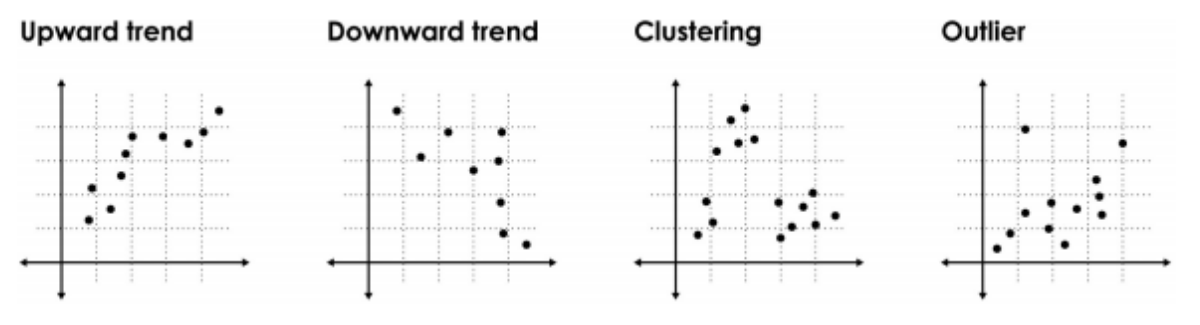
\includegraphics[scale=0.5]{005-1.png}
	\end{frame}

\begin{frame}{Aesthetics (Visual Cues): The Building Blocks}
	\begin{enumerate}
		\item Position (numerical): where in relation to other things? 
		\item Length (numerical): how big (in one dimension)? 
		\item  Angle (numerical): how wide? parallel to something else? 
		\item  Direction (numerical) at what slope? In a time series, going up or down? 
		\item  Shape (categorical) belonging to which group? 
		\item  Area (numerical) how big (in two dimensions)? 
		\item  Volume (numerical) how big (in three dimensions)? 
		\item  Shade (either) to what extent? how severely? 
		\item  Color (either) to what extent? how severely? Beware of red/green color blindness
		
		
	\end{enumerate}
\end{frame}


	\begin{frame}{Visual Cues: When you visualize data, you encode values to shapes, sizes, and colors}
		\centering
	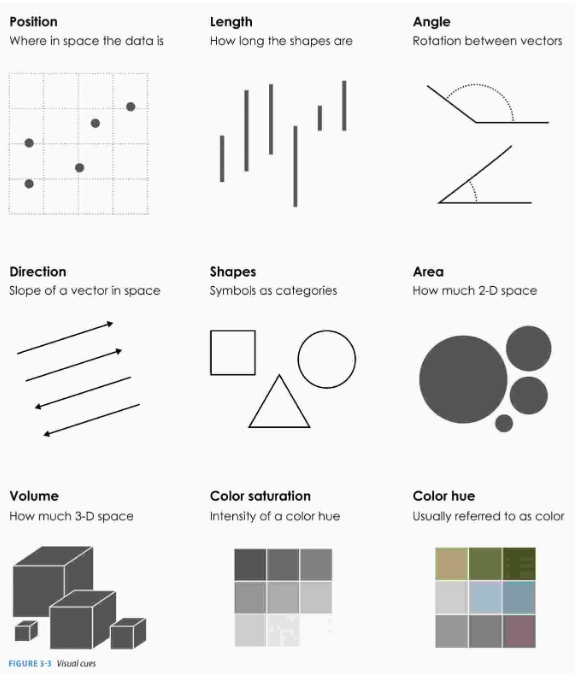
\includegraphics[scale=0.4]{005-2.png}
\end{frame}

	\begin{frame}{Commonly Used Visual Cues}
	\centering
	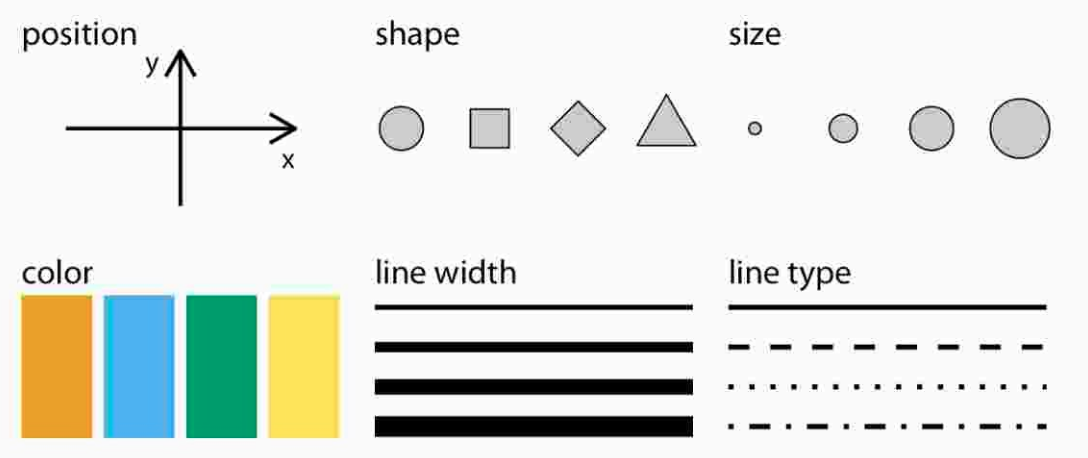
\includegraphics[scale=0.4]{005-3.png}
\end{frame}

	\begin{frame}{All visual cues fall into one of two groups}
\begin{itemize}
	\item Those that can represent continuous data and those that can not
\end{itemize}
\end{frame}


	\begin{frame}{Which of the following can represent continuous data? Discrete data?}
	\centering
	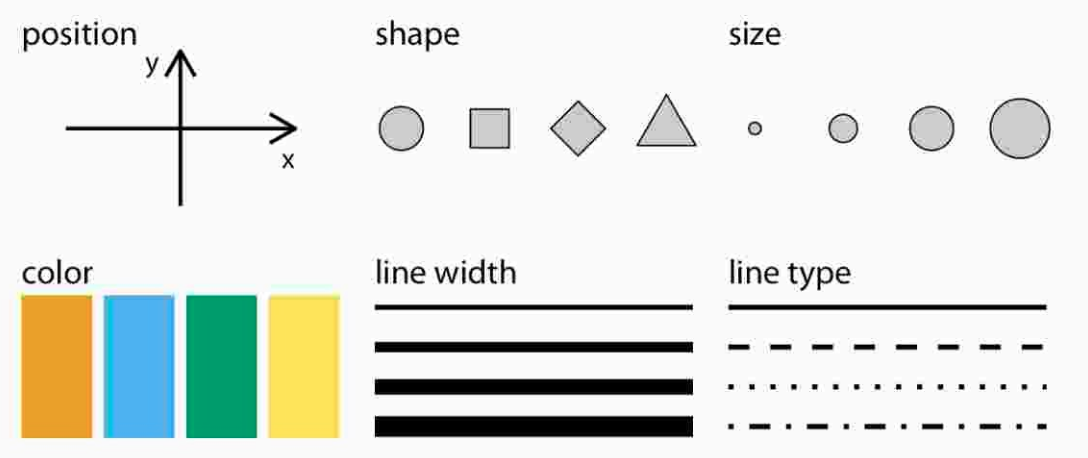
\includegraphics[scale=0.4]{005-3.png}
\end{frame}


\section{Scales}

\begin{frame}{Scales}
	\begin{itemize}
		\item To \textbf{map} data values onto \textbf{aesthetics}, we need to specify which data values correspond to which specific aesthetics values. \pause 
		\item For example, if our graphic has an x axis, then we need to specify which data values fall onto particular positions along this axis. \pause 
		\item Similarly, we may need to specify which data values are represented by particular shapes or colors. 
		
	\end{itemize}
\end{frame}


	\begin{frame}{Scales}
	\begin{itemize}
		\item This mapping between data values and aesthetics values is created via scales. 
		\item A scale defines a unique mapping between data and aesthetics.
		\item Importantly, \textbf{a scale must be one-to-one}, such that for each specific data value there is exactly one aesthetics value and vice versa. 
		\item If a scale isn't one-to-one, then the data visualization becomes ambiguous.		
	\end{itemize}
\end{frame}




	\begin{frame}{Scales}
		\begin{itemize}
			\item Scales link data values to aesthetics. 
			\item Here, the numbers 1 through 4 have been mapped onto a position scale, a shape scale, and a color scale. 
			\item For each scale, each number corresponds to a unique position, shape, or color and vice versa
		\end{itemize}
	\centering
	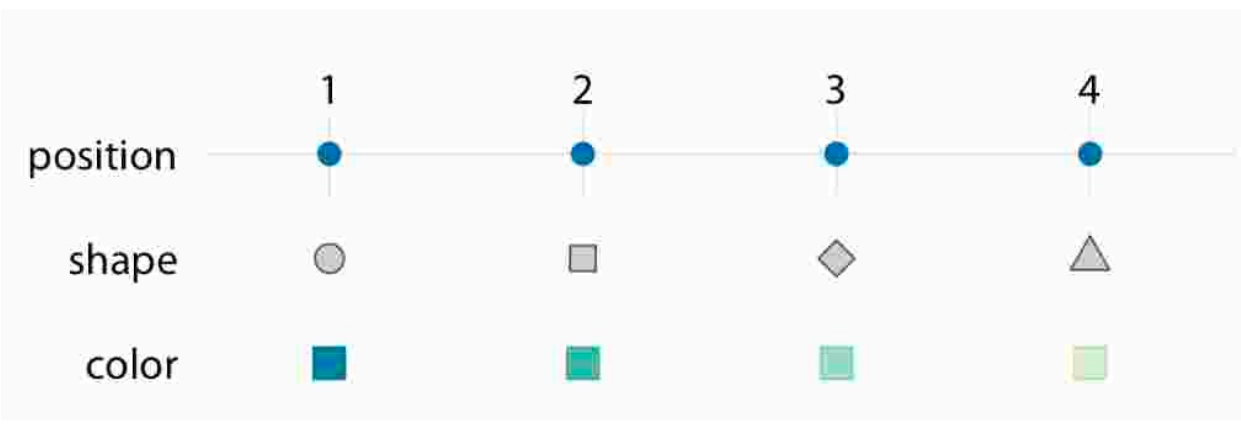
\includegraphics[scale=0.3]{005-5.png}
\end{frame}


	\begin{frame}{How many scales are being used?}
	\centering
	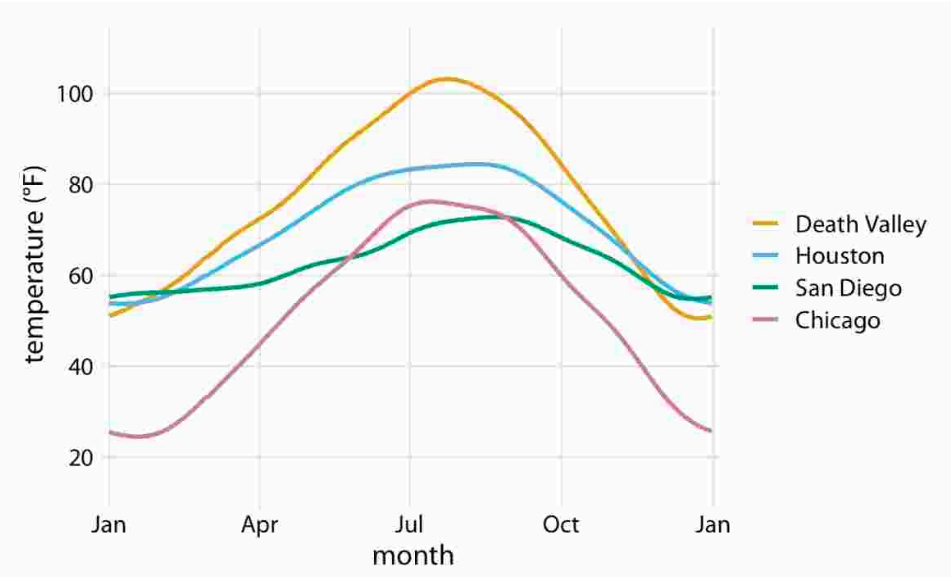
\includegraphics[scale=0.4]{005-6.png}
\end{frame}

	\begin{frame}{How many scales are being used?}
	\centering
	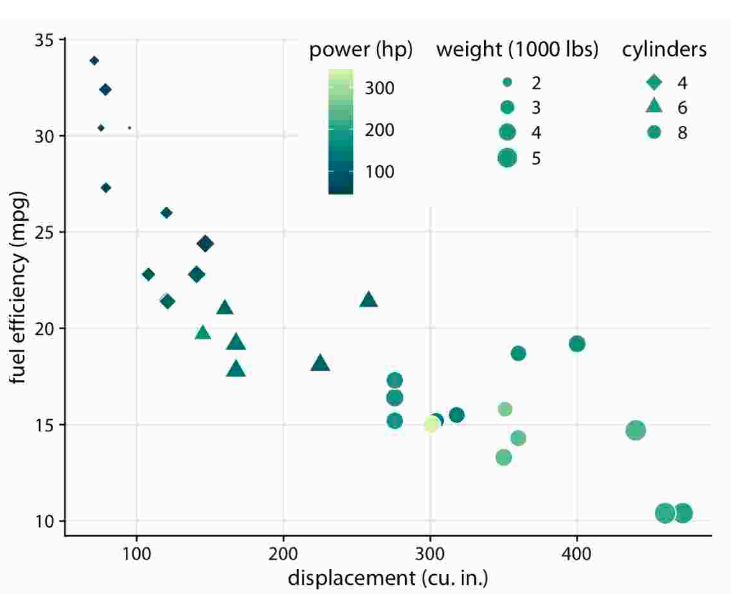
\includegraphics[scale=0.4]{005-7.png}
\end{frame}

	\begin{frame}{How many scales are being used?}
	\centering
	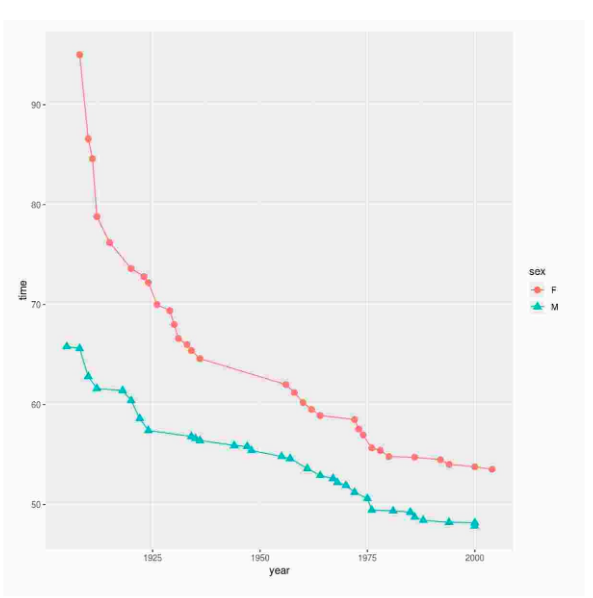
\includegraphics[scale=0.4]{005-8.png}
\end{frame}


\begin{frame}{Difference between Aesthetics (Visual Cues) and Scales ?}
\begin{itemize}
	\item \textbf{Aesthetics:} describe every aspect of a given graphical element.
	\item \textbf{Scale:} defines a unique mapping between data and aesthetics.
	\item A scale is a visual cue with data attached to it
	
\end{itemize}
\end{frame}


\section{Color scales}

\begin{frame}{Color scales: 3 use cases}
	\begin{enumerate}
		\item To distinguish groups of data from each other
		\item Represent data values
		\item To highlight
	\end{enumerate}

\vspace{0.2in}
		The types of colors we use and the way in which we use them are quite different for these three cases.
\end{frame}


	\begin{frame}{Color as a tool to distinguish}
	\centering
	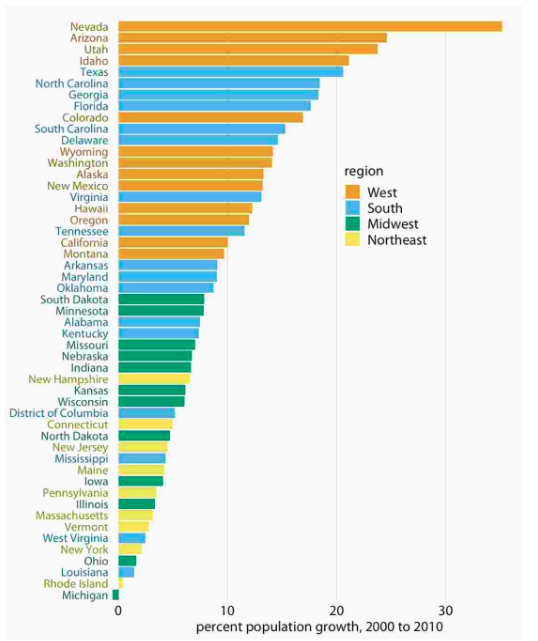
\includegraphics[scale=0.4]{005-9.png}
\end{frame}


	\begin{frame}{Color to represent values}
	\centering
	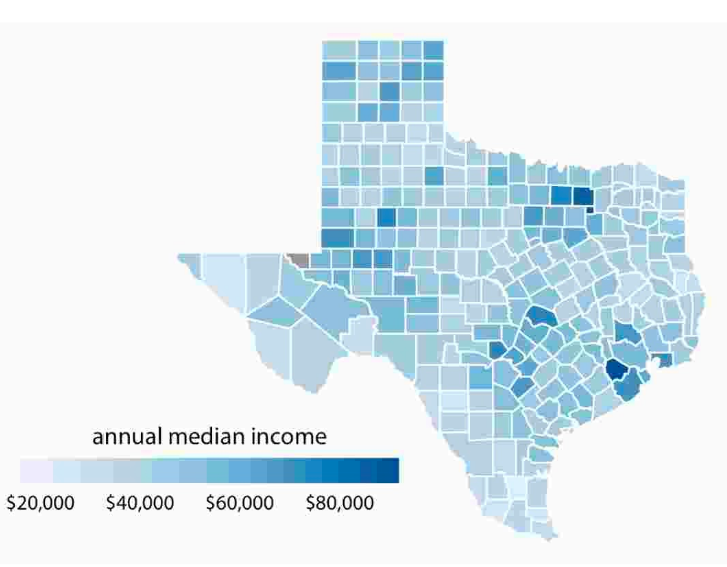
\includegraphics[scale=0.4]{005-10.png}
\end{frame}


	\begin{frame}{Color as a tool to highlight}
	\centering
	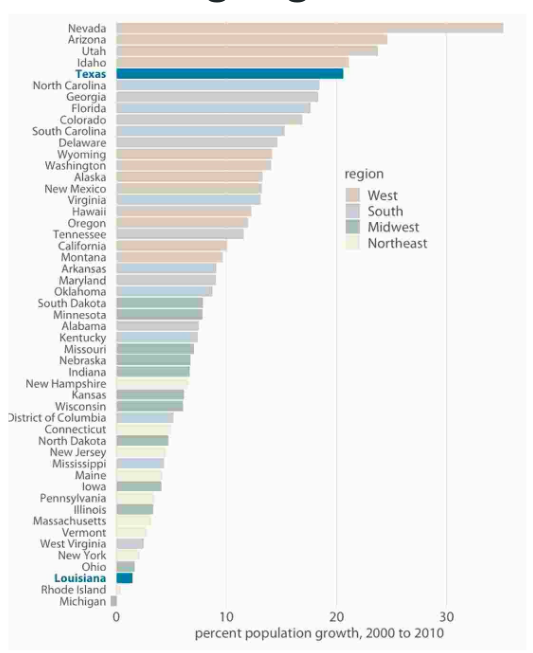
\includegraphics[scale=0.4]{005-11.png}
\end{frame}



	\begin{frame}{Cynthia Brewer Palette}
	\centering
	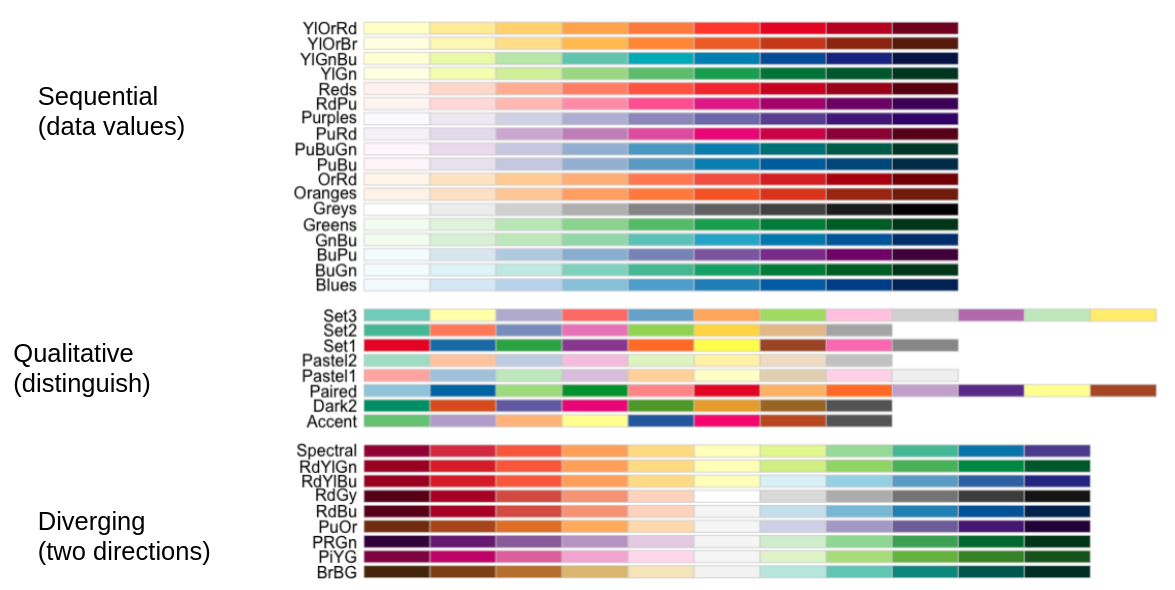
\includegraphics[scale=0.4]{005-12.png}
\end{frame}


	\begin{frame}{Good choice of colors?}
	\centering
	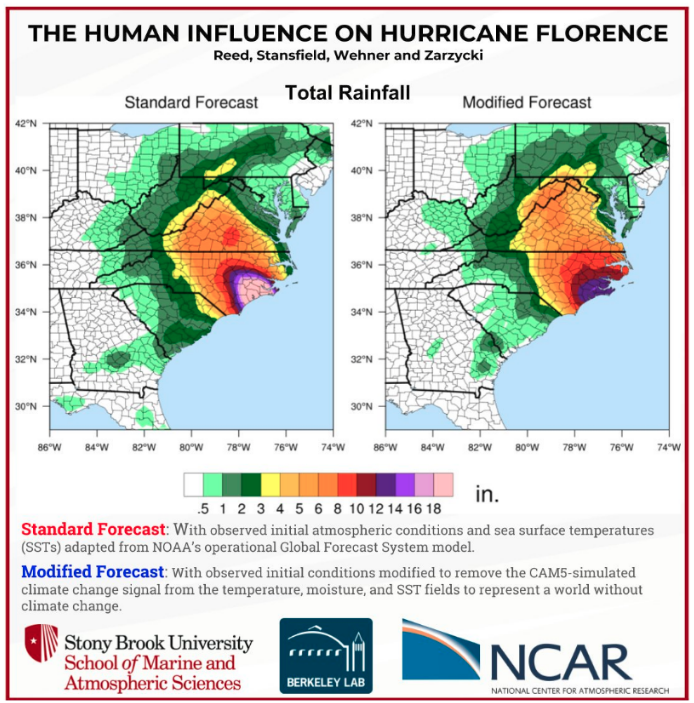
\includegraphics[scale=0.4]{005-13.png}
\end{frame}




	\begin{frame}{Perceptually Uniform Palettes}
	\centering
	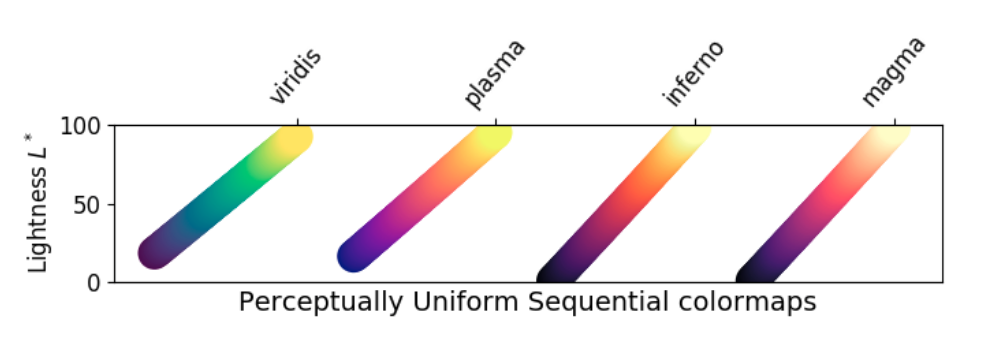
\includegraphics[scale=0.4]{005-14.png}
	
	\begin{itemize}
		\item \url{https://cran.r-project.org/web/packages/colorspace/vignettes/colorspace.html}
		\item \url{https://cran.r-project.org/web/packages/viridis/vignettes/intro-to-viridis.html}
	\end{itemize}
\end{frame}



\begin{frame}[fragile]{Qualitative palette}
\begin{knitrout}\tiny
\definecolor{shadecolor}{rgb}{0.969, 0.969, 0.969}\color{fgcolor}\begin{kframe}
\begin{alltt}
\hlkwd{library}\hlstd{(oibiostat);} \hlkwd{data}\hlstd{(}\hlstr{"famuss"}\hlstd{)}
\hlkwd{library}\hlstd{(ggplot2)}
\hlkwd{library}\hlstd{(colorspace)}

\hlkwd{ggplot}\hlstd{(famuss,} \hlkwd{aes}\hlstd{(}\hlkwc{x} \hlstd{= actn3.r577x,} \hlkwc{y} \hlstd{= bmi,} \hlkwc{fill} \hlstd{= actn3.r577x))} \hlopt{+}
  \hlkwd{geom_boxplot}\hlstd{()} \hlopt{+}
  \hlstd{colorspace}\hlopt{::}\hlkwd{scale_fill_discrete_qualitative}\hlstd{()}
\end{alltt}
\end{kframe}

{\centering 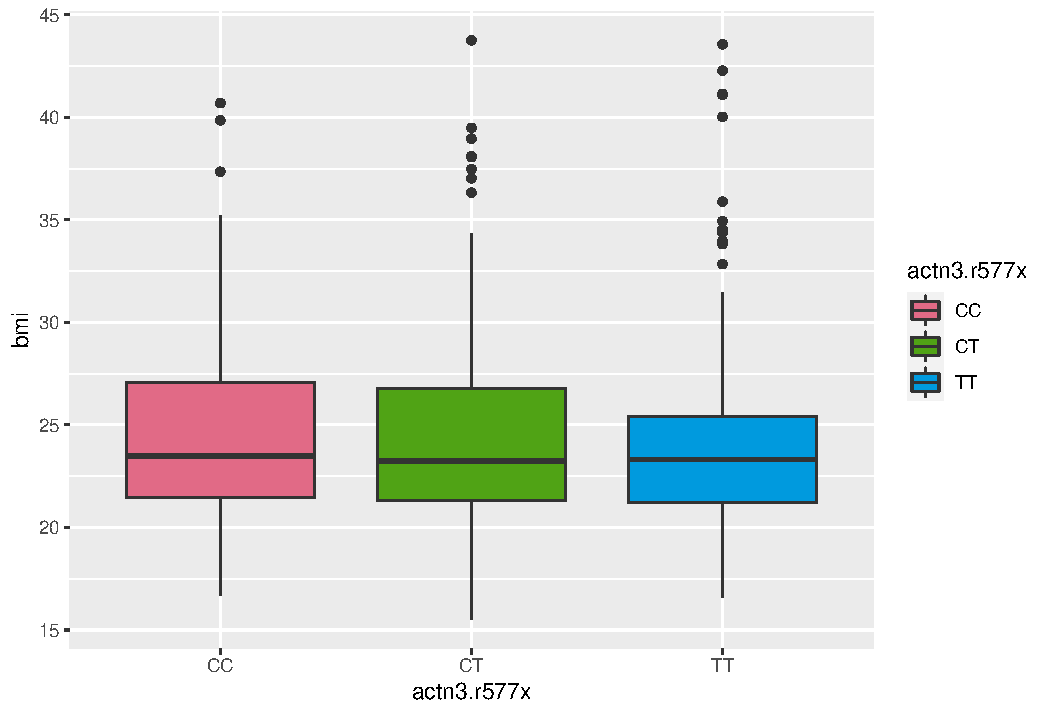
\includegraphics[width=\maxwidth]{figure/unnamed-chunk-1-1} 

}


\begin{kframe}\begin{alltt}
\hlkwd{ggplot}\hlstd{(famuss,} \hlkwd{aes}\hlstd{(}\hlkwc{x} \hlstd{= height,} \hlkwc{y} \hlstd{= weight,} \hlkwc{color} \hlstd{= bmi))} \hlopt{+}
  \hlkwd{geom_point}\hlstd{()} \hlopt{+}
  \hlstd{colorspace}\hlopt{::}\hlkwd{scale_color_continuous_sequential}\hlstd{(}\hlkwc{palette} \hlstd{=} \hlstr{"Viridis"}\hlstd{)}
\end{alltt}
\end{kframe}

{\centering 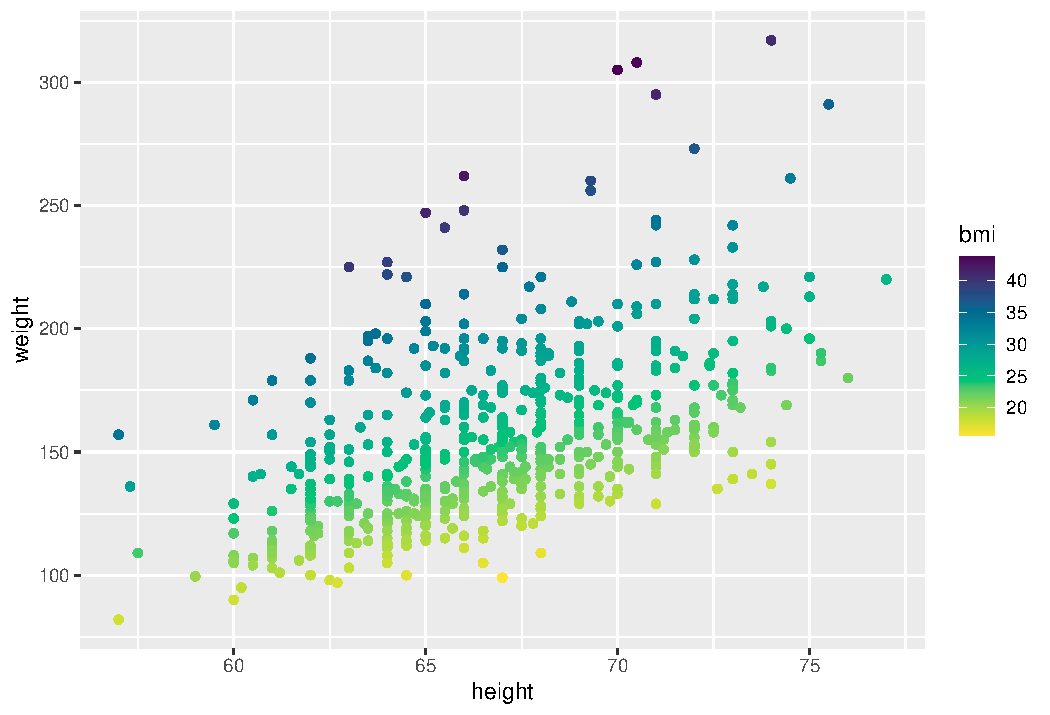
\includegraphics[width=\maxwidth]{figure/unnamed-chunk-1-2} 

}



\end{knitrout}
\end{frame}

	
	
	\begin{frame}[fragile]{Sequential palette}
\begin{knitrout}\tiny
\definecolor{shadecolor}{rgb}{0.969, 0.969, 0.969}\color{fgcolor}\begin{kframe}
\begin{alltt}
\hlkwd{ggplot}\hlstd{(famuss,} \hlkwd{aes}\hlstd{(}\hlkwc{x} \hlstd{= height,} \hlkwc{y} \hlstd{= weight,} \hlkwc{color} \hlstd{= bmi))} \hlopt{+}
  \hlkwd{geom_point}\hlstd{()} \hlopt{+}
  \hlstd{colorspace}\hlopt{::}\hlkwd{scale_color_continuous_sequential}\hlstd{(}\hlkwc{palette} \hlstd{=} \hlstr{"Viridis"}\hlstd{)}
\end{alltt}
\end{kframe}

{\centering 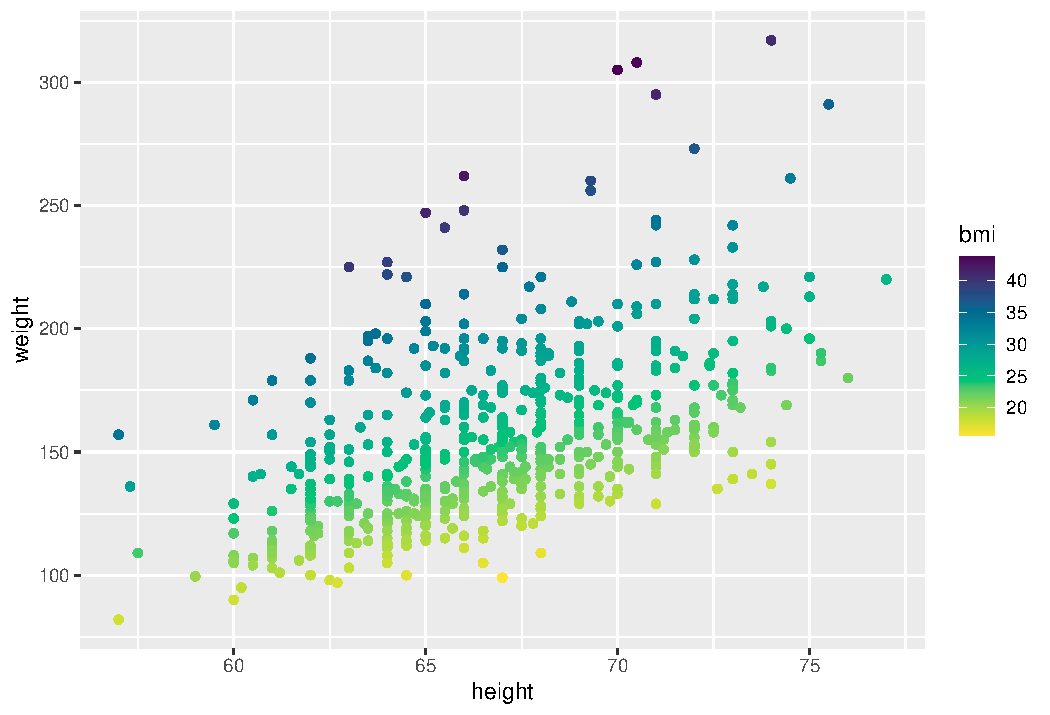
\includegraphics[width=\maxwidth]{figure/unnamed-chunk-2-1} 

}



\end{knitrout}
	\end{frame}
	
	
	\begin{frame}[fragile]{Session Info}
		\tiny
		
\begin{knitrout}\tiny
\definecolor{shadecolor}{rgb}{0.969, 0.969, 0.969}\color{fgcolor}\begin{kframe}
\begin{verbatim}
R version 3.6.2 (2019-12-12)
Platform: x86_64-pc-linux-gnu (64-bit)
Running under: Pop!_OS 19.10

Matrix products: default
BLAS:   /usr/lib/x86_64-linux-gnu/openblas/libblas.so.3
LAPACK: /usr/lib/x86_64-linux-gnu/libopenblasp-r0.3.7.so

attached base packages:
[1] tools     stats     graphics  grDevices utils     datasets  methods  
[8] base     

other attached packages:
 [1] colorspace_1.4-1   oibiostat_0.2.0    NCStats_0.4.7      FSA_0.8.30        
 [5] forcats_0.5.0      stringr_1.4.0      dplyr_1.0.2        purrr_0.3.4       
 [9] readr_1.3.1        tidyr_1.1.2        tibble_3.0.3       ggplot2_3.3.2.9000
[13] tidyverse_1.3.0    knitr_1.29        

loaded via a namespace (and not attached):
 [1] tidyselect_1.1.0   xfun_0.16          haven_2.3.1        vctrs_0.3.4       
 [5] generics_0.0.2     rlang_0.4.7        pillar_1.4.6       glue_1.4.2        
 [9] withr_2.2.0        DBI_1.1.0          dbplyr_1.4.2       modelr_0.1.5      
[13] readxl_1.3.1       lifecycle_0.2.0    plyr_1.8.6         munsell_0.5.0     
[17] gtable_0.3.0       cellranger_1.1.0   rvest_0.3.5        evaluate_0.14     
[21] labeling_0.3       fansi_0.4.1        highr_0.8          broom_0.7.0       
[25] Rcpp_1.0.4.6       scales_1.1.1       backports_1.1.9    jsonlite_1.7.0    
[29] farver_2.0.3       fs_1.3.2           TeachingDemos_2.12 hms_0.5.3         
[33] digest_0.6.25      stringi_1.4.6      grid_3.6.2         cli_2.0.2         
[37] magrittr_1.5       crayon_1.3.4       pkgconfig_2.0.3    ellipsis_0.3.1    
[41] xml2_1.3.0         reprex_0.3.0       lubridate_1.7.4    assertthat_0.2.1  
[45] httr_1.4.1         rstudioapi_0.11    R6_2.4.1           compiler_3.6.2    
\end{verbatim}
\end{kframe}
\end{knitrout}
		
	\end{frame}
	
\end{document}
